\section*{Question 1}
The optimal solution to the provided LP solution was found using the Microsoft Excel Solver. The LP model setup in Excel can be seen in Figure~\ref{fig:q1_model}. The optimal solution is found using the Excel Solver with Simplex LP Solving Method. The optimal solution is [X$_1$ = 0, X$_2$ = 11.5, X$_3$ = 14.8, X$_4$ = 10.4] with Max Z = 889.3, as seen in Figure~\ref{fig:q1_answer}.

The acceptable range for the cost coefficients are:
\begin{gather*}
	-\infty \leq C_1 \leq 29.1 \\
	6.8 \leq C_2 \leq 86.4 \\
	33.17 \leq C_3 \leq \infty \\
	-\infty \leq C_4 \leq 32.5
\end{gather*}

The acceptable range for the stipulations are:
\begin{gather*}
	153.33 \leq B_1 \leq 230 \\
	50.01 \leq B_2 \leq \infty \\
	0 \leq B_3 \leq 35.33 \\
	33 \leq B_4 \leq 56.57
\end{gather*}

The Excel spreadsheet is included with the assignment submission as \texttt{question1.xlsx}.

\begin{figure}[htp]
    \centering
    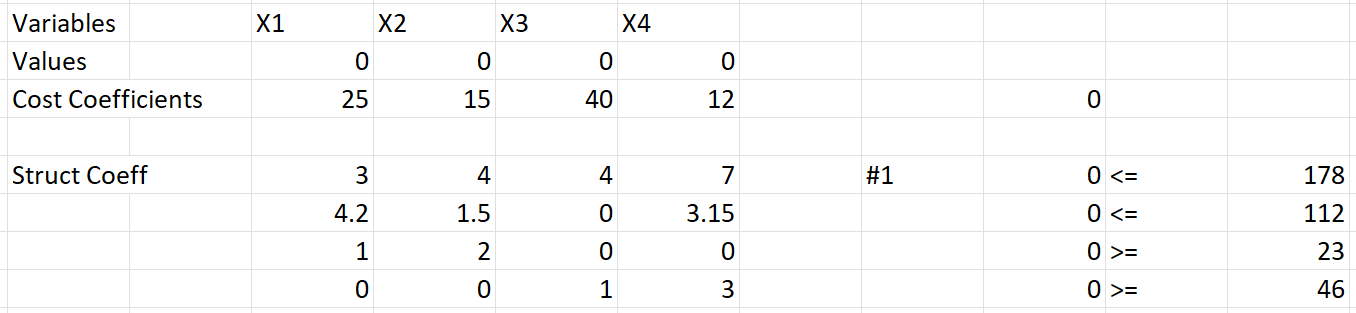
\includegraphics[width=0.9\textwidth]{1_model.png}
    \caption{\label{fig:q1_model}Excel Solver Model}
\end{figure}

\begin{figure}[htp]
    \centering
    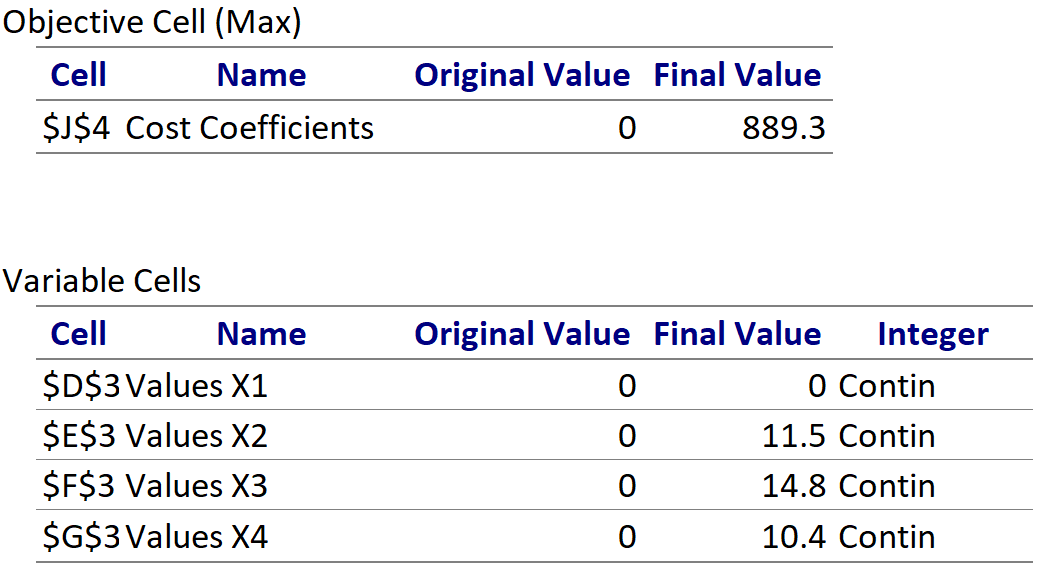
\includegraphics[width=0.45\textwidth]{1_solution.png}
    \caption{\label{fig:q1_answer}Excel Solver Solution}
\end{figure}

\begin{figure}[htp]
    \centering
    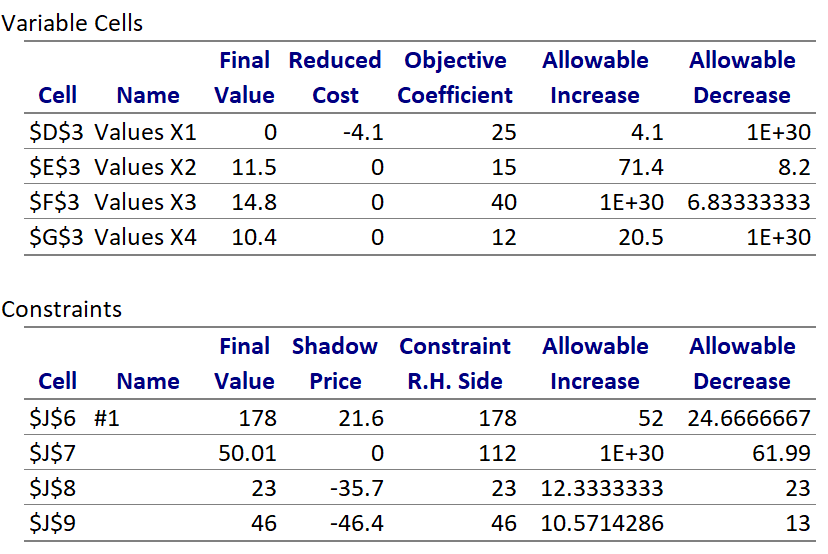
\includegraphics[width=0.52\textwidth]{1_sensitivity.png}
    \caption{\label{fig:q1_sensitivity}Excel Solver Sensitivity}
\end{figure}